%%%%%%%%%%%%%%%%%%%%%%%%%%%%%%%%%%%%%%%%%%%%%%%%%%%%%%%%%%%%%%%
%
% Introduction.tex (part of thesis.tex)
% author: Qie Hu
%
%%%%%%%%%%%%%%%%%%%%%%%%%%%%%%%%%%%%%%%%%%%%%%%%%%%%%%%%%%%%%%%

%!TEX root = ../../thesis.tex

\section{Model Identification}\label{sec:model_id}

\subsection{Building Model}
The data-driven model identified for the fourth floor of SDH in Chapter \ref{chapter:building_model} is used here in our field experiments.
To recap, we model the room temperature evolution as follows:
\begin{equation}
\begin{aligned}\label{eq:building_model}
x(k+1) &= A x(k) + B u(k) + C v(k) + q(k), \\
\end{aligned}
\end{equation}
where $x \in \mathbb{R}^6$ represents the average temperature in each of the six zones on the fourth floor (see Figure \ref{fig:floor_plan}), $u \in \mathbb{R}^6$ contains the total airflow to each zone, $v:= \left[ v_\text{Ta}, v_\text{Ts} \right]^\top \in \mathbb{R}^2$ is a disturbance vector that describes ambient air temperature and the HVAC system's SAT and  $q \in \mathbb{R}^6$ contains internal gains due to occupancy and electric devices in each zone.
Finally, $A$, $B \in \mathbb{R}^{6\times6}$ and $C \in \mathbb{R}^{6\times2}$ are coefficient matrices.


%%%%%%%%%%%%%%%%%%%%%%%%%%%%%%%%%%%%%%%%%%%%%%
%%%%%%%%%%%%%%%%%%%%%%%%%%%%%%%%%%%%%%%%%%%%%%
%%%%%%%%%%%%%%%%%%%%%%%%%%%%%%%%%%%%%%%%%%%%%%
%%%%%%%%%%%%%%%%%%%%%%%%%%%%%%%%%%%%%%%%%%%%%%


\subsection{Fan Model}

SDH's HVAC system contains two AHUs, each of them houses a set of supply fans that operate at the same speed at all times.
In this work, we model the fans in both AHUs as a single unit, i.e., we control them to the same fan speed, we consider their total power consumption and the total air flow rate through both AHUs.
With this setup, a fan model is identified from 6 weeks of one-minute resolution data collected from sMAP.
The fan laws state that the airflow rate through the fan is proportional to the fan speed, and the fan power is a cubic function of its speed \cite{Hvac_book}. 
Figure \ref{fig:fan_model} confirms the linear relationship between the airflow rate and the fan speed.
It also shows that for the range of fan speeds used in this work (i.e., 20\% to 60\% of maximum fan speed), a quadratic function can describe the relationship between fan power and fan speed without significant loss of accuracy compared to a cubic function, and %for fan speed between 28\% and 90\% of its maximum.
since a quadratic function would simplify the subsequent controller design problem, it is adopted in this work. 
%Assume both supply fans are controlled to the same speed. 
%Let $N$ denote the fan speed of both fans, $u$ the total airflow rate through the fans and $P$ the total power consumption of the fans, then the fan model is defined as follows:

Let $N$ denote the fan speed, $u$ the total airflow through the fans and $P$ the total fan power consumption, then the fan model is given as follows:
\begin{equation}\label{eq:fan_model}
\begin{aligned}
N & = f(u) = a_1 u + a_2\\
P & = g(N) = b_1 N^2 + b_2 N + b_3\\
P & = h(u) = c_1 u^2 + c_2 u + c_3.\\
\end{aligned}
\end{equation} 

\begin{figure}[h]
\centering
\vspace*{1cm}
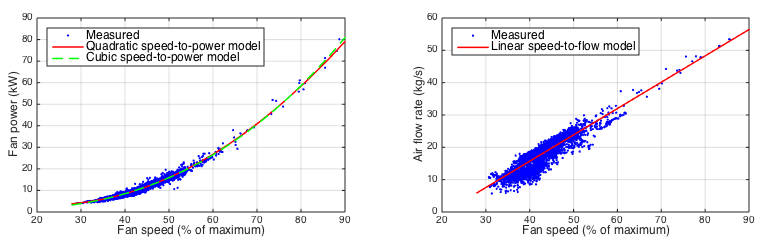
\includegraphics[width=\textwidth]{chapters/building_exp/figures/fan_model.png}
\caption{Fan measurements and identified models for fan power and air flow as functions of fan speed.}
\label{fig:fan_model}
\vspace*{1cm}
\end{figure}








